\section{Experiments}\label{sec:experiments}
We said that zero-knowledge provable computation is especially interesting in blockchain
environments, like cryptocurrencies, where users commit to transactions by means of a tree-mode of
hash.
We implemented and tested several combinations of cryptographic primitives for tree-path
verification, using the C\texttt{++} language and the facilities based on the Pinocchio protocol
provided by the \texttt{libsnark} library.
In particular, we implemented:
\begin{itemize}
	\item Hash-agnostic Merkle trees.
	\item Hash-agnostic ABRs.
	\item SHA-256 (adapted from the versionprovided by \texttt{libsnark}) and SHA-512.
	\item \(1/2/1\) MiMC-256, single and double key MiMC-512 Feistel (MiMC-512F) OWCFs
	      over prime fields.
\end{itemize}

\noindent Since the computational complexity of Pinocchio is basically defined by the number of
multiplications in the arithmetic circuit, we can predict the expected performance of the various
hash modes.
Given some \(n\)-bit hash function \(H\) and its arithmetic circuit \(\phi\left(H\right)\), the
Merkle tree \(\mathcal{T}_H\) of height \(h\) and the path checking arithmetic circuit
\(\phi\left(\mathcal{T}_H\right)\), then:
\[
	\left|{\phi\left(\mathcal{T}_H\right)}_\otimes\right| =
	\left(h-1\right)\left|{\phi\left(H\right)}_\otimes\right|
\]
If we consider an ABR \(\mathcal{A}_H\) of the same height, the complexity of the \(\otimes \)
operations depends on whether \(H\) works natively over a prime field or a binary field.
In the former case:
\[
	\left|{\phi\left(\mathcal{A}_H\right)}_\otimes\right| = \left|{\phi\left(H\right)}_\otimes\right|
	+ \left(h-2\right)\left(3 + \left|{\phi\left(H\right)}_\otimes\right|\right)
\]
In the latter case:
\[
	\left|{\phi\left(\mathcal{A}'_H\right)}_\otimes\right| = \left|{\phi\left(H\right)}_\otimes\right|
	+ \left(h-2\right)\left(3n + \left|{\phi\left(H\right)}_\otimes\right|\right) + 2n\left(h-1\right)
\]
If we compare the multiplication complexity of \(\mathcal{T}_H\) and \(\mathcal{A}_H\), we get:
\[
	\frac{\left|{\phi\left(\mathcal{A}_H\right)}_\otimes\right|}
	{\left|{\phi\left(\mathcal{T}_H\right)}_\otimes\right|} =
	1 + 3\left(\frac{1}{\left|{\phi\left(H\right)}_\otimes\right|} -
	\frac{1}{\left(h-1\right)\left|{\phi\left(H\right)}_\otimes\right|}\right) \approx 1
\]
Tipically, \(\left|{\phi\left(H\right)}_\otimes\right| > 10^2\), so the 25\% increment in
density offered by ABRs over Merkle Trees comes at a negligible cost w.r.t.\ multiplicative
complexity, as long as \(\oplus \) is intended over the native ZK-SNARK field.
\begin{table}
	\centering
	\begin{tabular}{cccc}
		\toprule
		Name         & Rounds & muls/round       & tot.\ muls         \\
		\midrule
		SHA-256      & 64     & \(\approx 512\)  & \(\approx 43776\)  \\
		SHA-512      & 80     & \(\approx 1024\) & \(\approx 111104\) \\
		MiMC-256     & 160    & 2                & 639                \\
		SK-MiMC-512F & 320    & 2                & 2558               \\
		DK-MiMC-512F & 400    & 2                & 1598               \\
		\bottomrule
	\end{tabular}
	\caption{Multiplicative complexity of the implemented hash functions.
		The `tot.\ muls' column counts multiplications independent from the number of rounds, and
		ones dependent on the construction (e.g.\ Davies Meyer).}\label{tab:hash_mulcomp}
\end{table}
Table~\ref{tab:hash_mulcomp} shows the multiplicative complexity of the hash functions under study.
It is likely that the values for SHA-256 and SHA-512 can be significantly optimized, but are still
in the range of the tens of thousands, with SHA-512 requiring \(\approx 2.5\times \) more
multiplications than SHA-256.
Tests of our implementations confirm our calculations.
\begin{figure}[t]
	\centering
	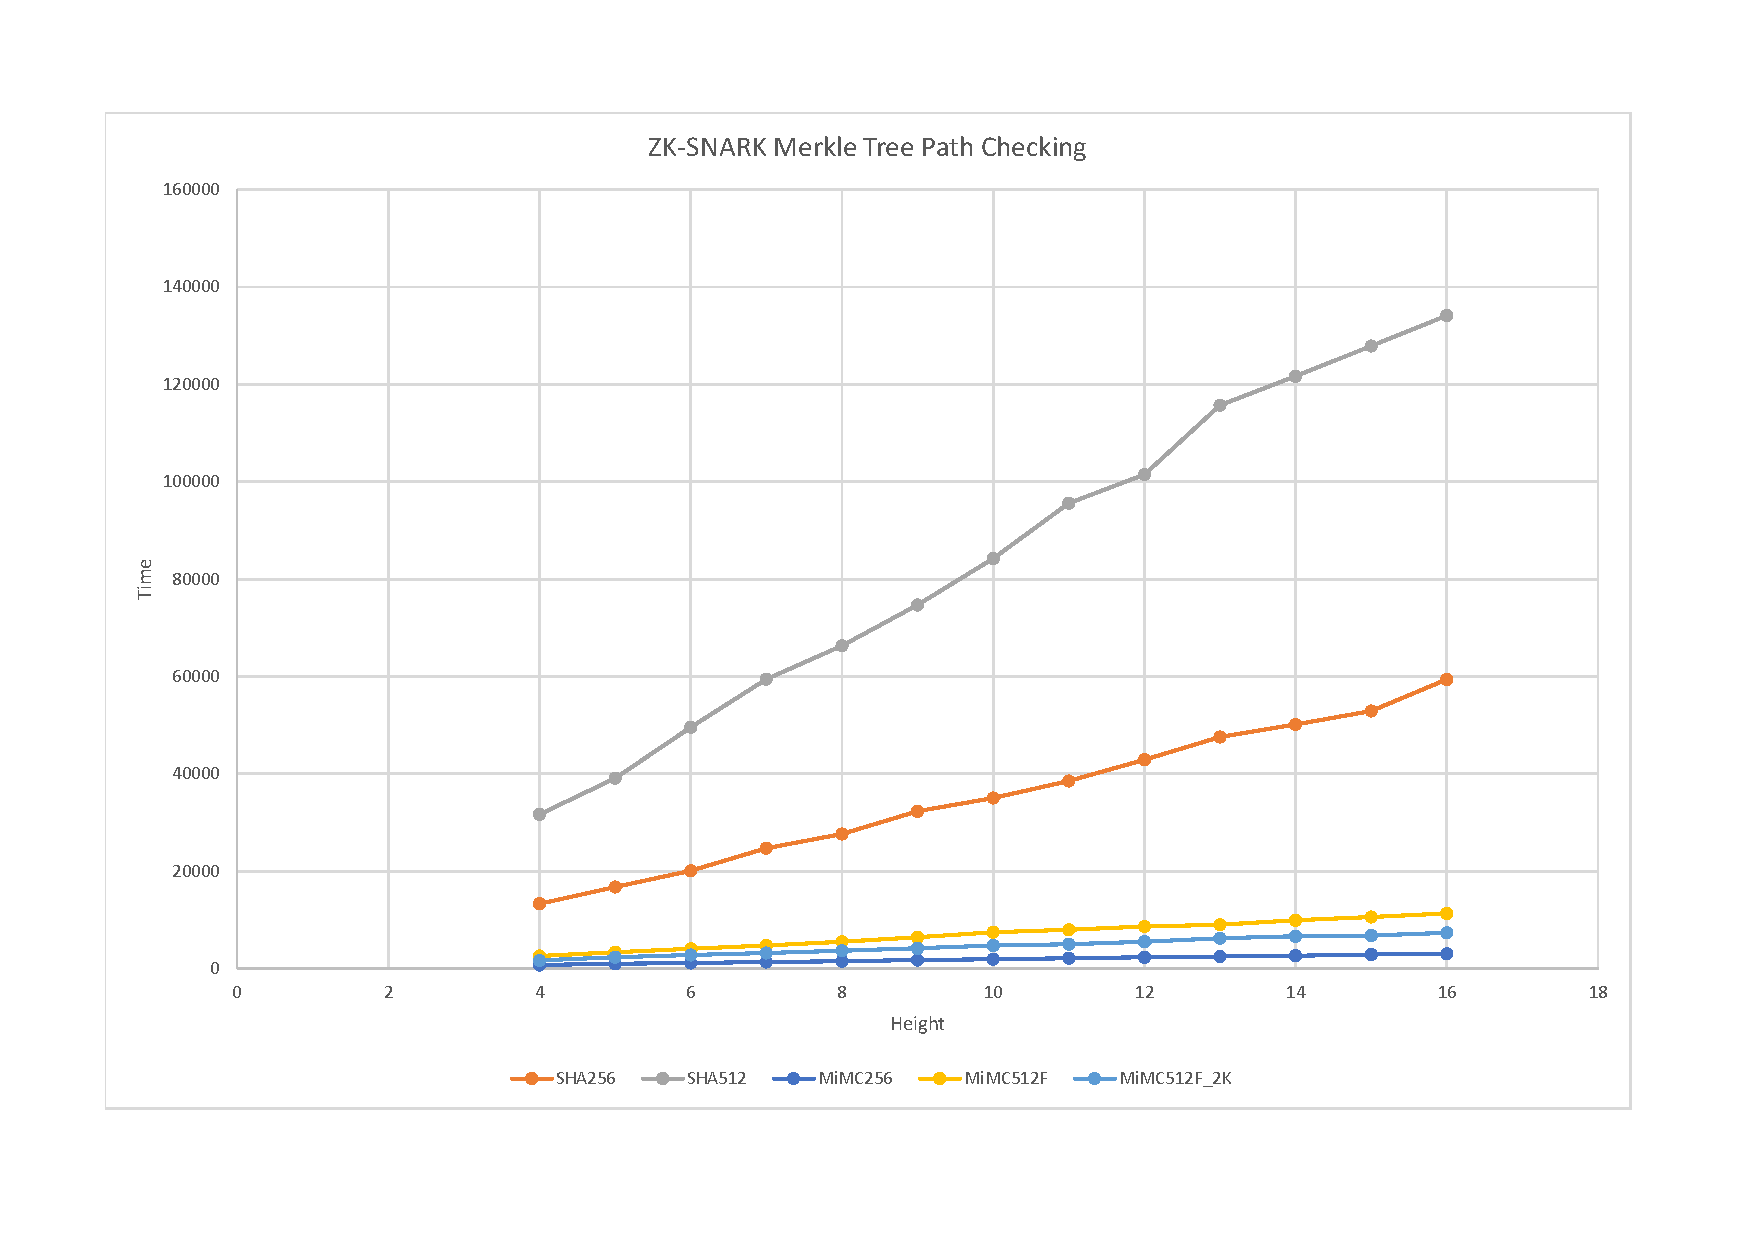
\includegraphics[scale=0.33]{res/mtree_total.pdf}
	\caption{Total time (in ms) required for synthesizing and solving a ZK-SNARK Merkle Tree path
		veritication circuit at varying heights.}\label{fig:mtree_total}
\end{figure}

Figure~\ref{fig:mtree_total} shows the total time, in milliseconds, required to create an
arithmetic circuit for Merkle tree path verification, convert it to R1CS, build the QAP and the
proof, and verify the proof, using different underlying hash functions.
As expected, MiMC-256 is the fastest one, followed by double-key MiMC-512F and single-key MiMC-512F
in the respective order, with SHA-256 and SHA-512 being extremely slower.
\begin{figure}
	\centering
	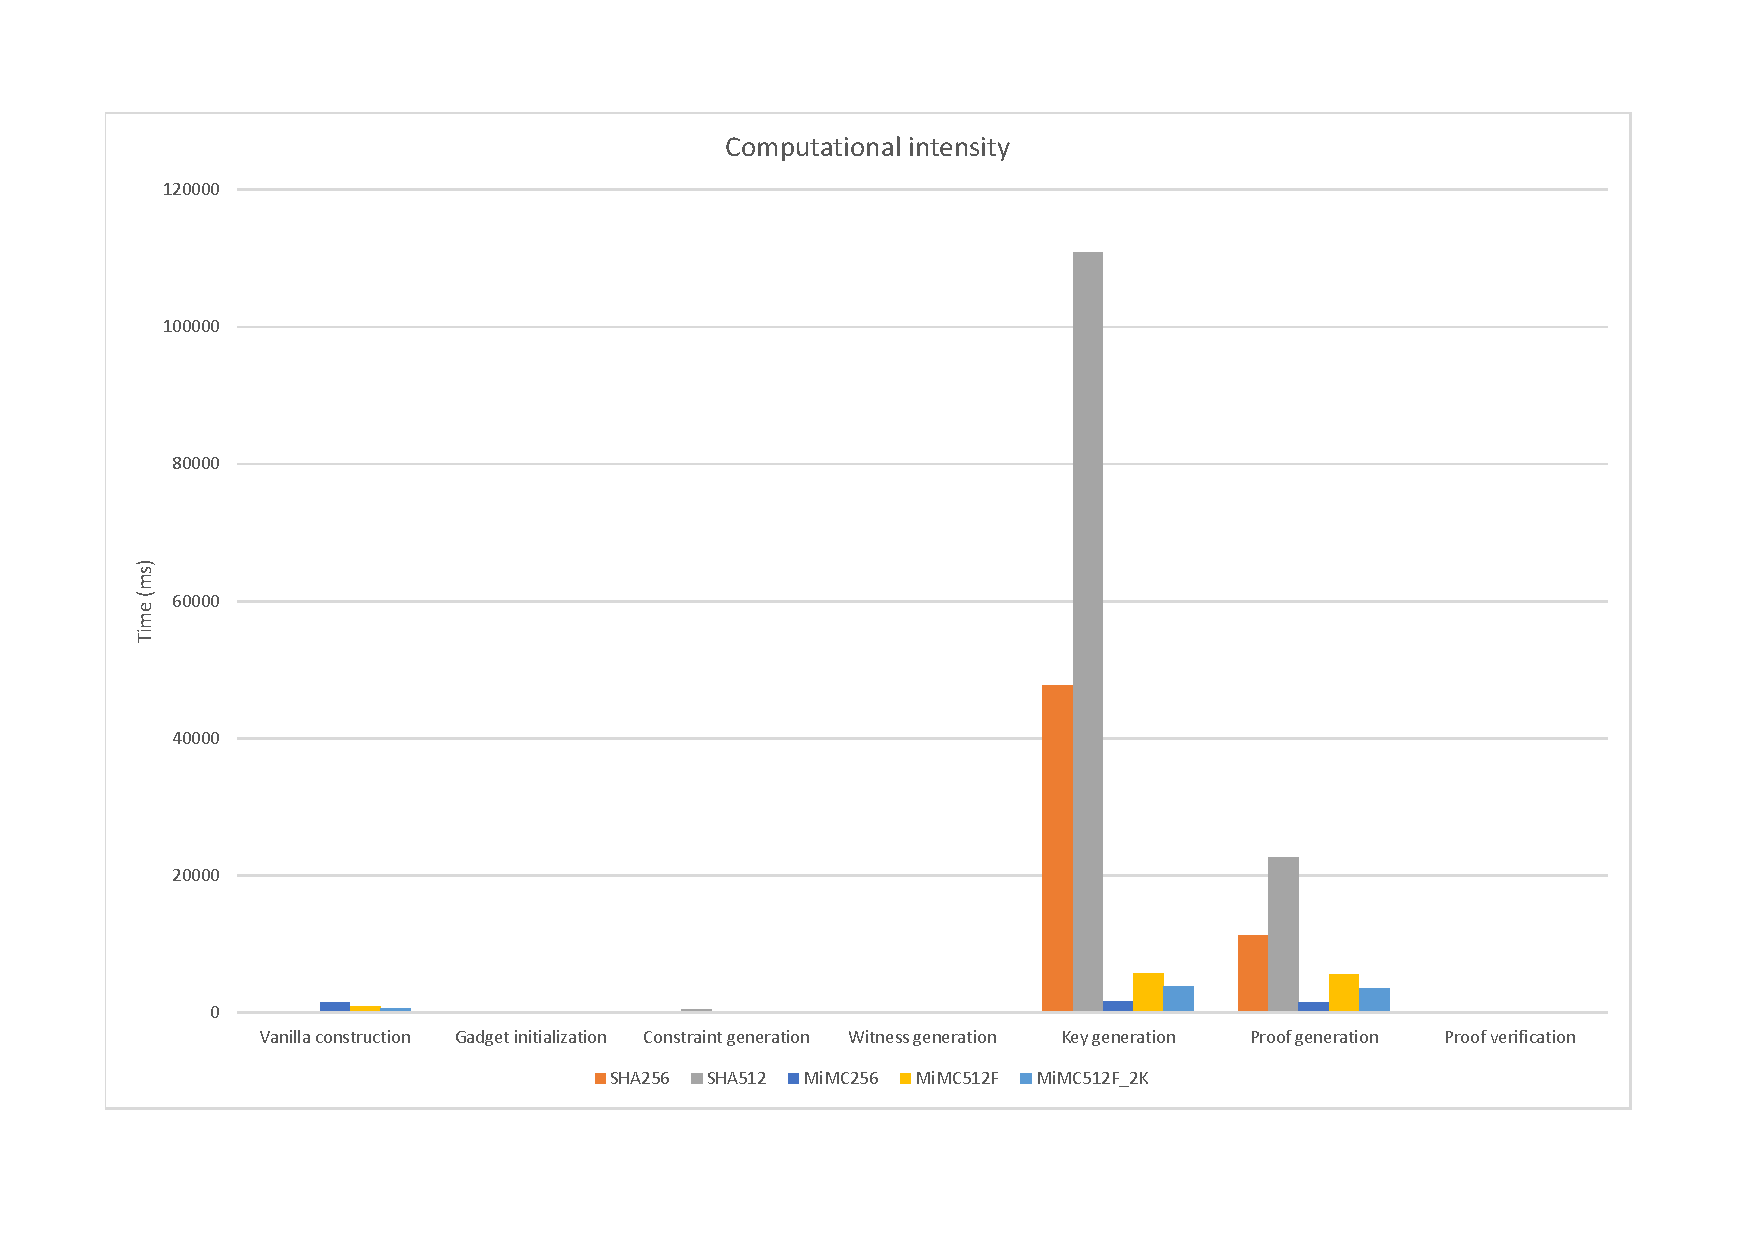
\includegraphics[scale=0.33]{res/mtree_intensity.pdf}
	\caption{Computational intensity of the various phases of the ZK-SNARK protocol: key and proof
		generation dominate the cost.}\label{fig:mtree_intensity}
\end{figure}

Figure~\ref{fig:mtree_intensity} shows the computational intensity of the different parts of the
Pinocchio protocol: since key and proof generation times completely dominate the cost, and these
are transparent to the library user, it is extremely important to optimize the arithmetic circuit
layout, even if it makes the synthesizing code more complex.
\begin{figure}
	\centering
	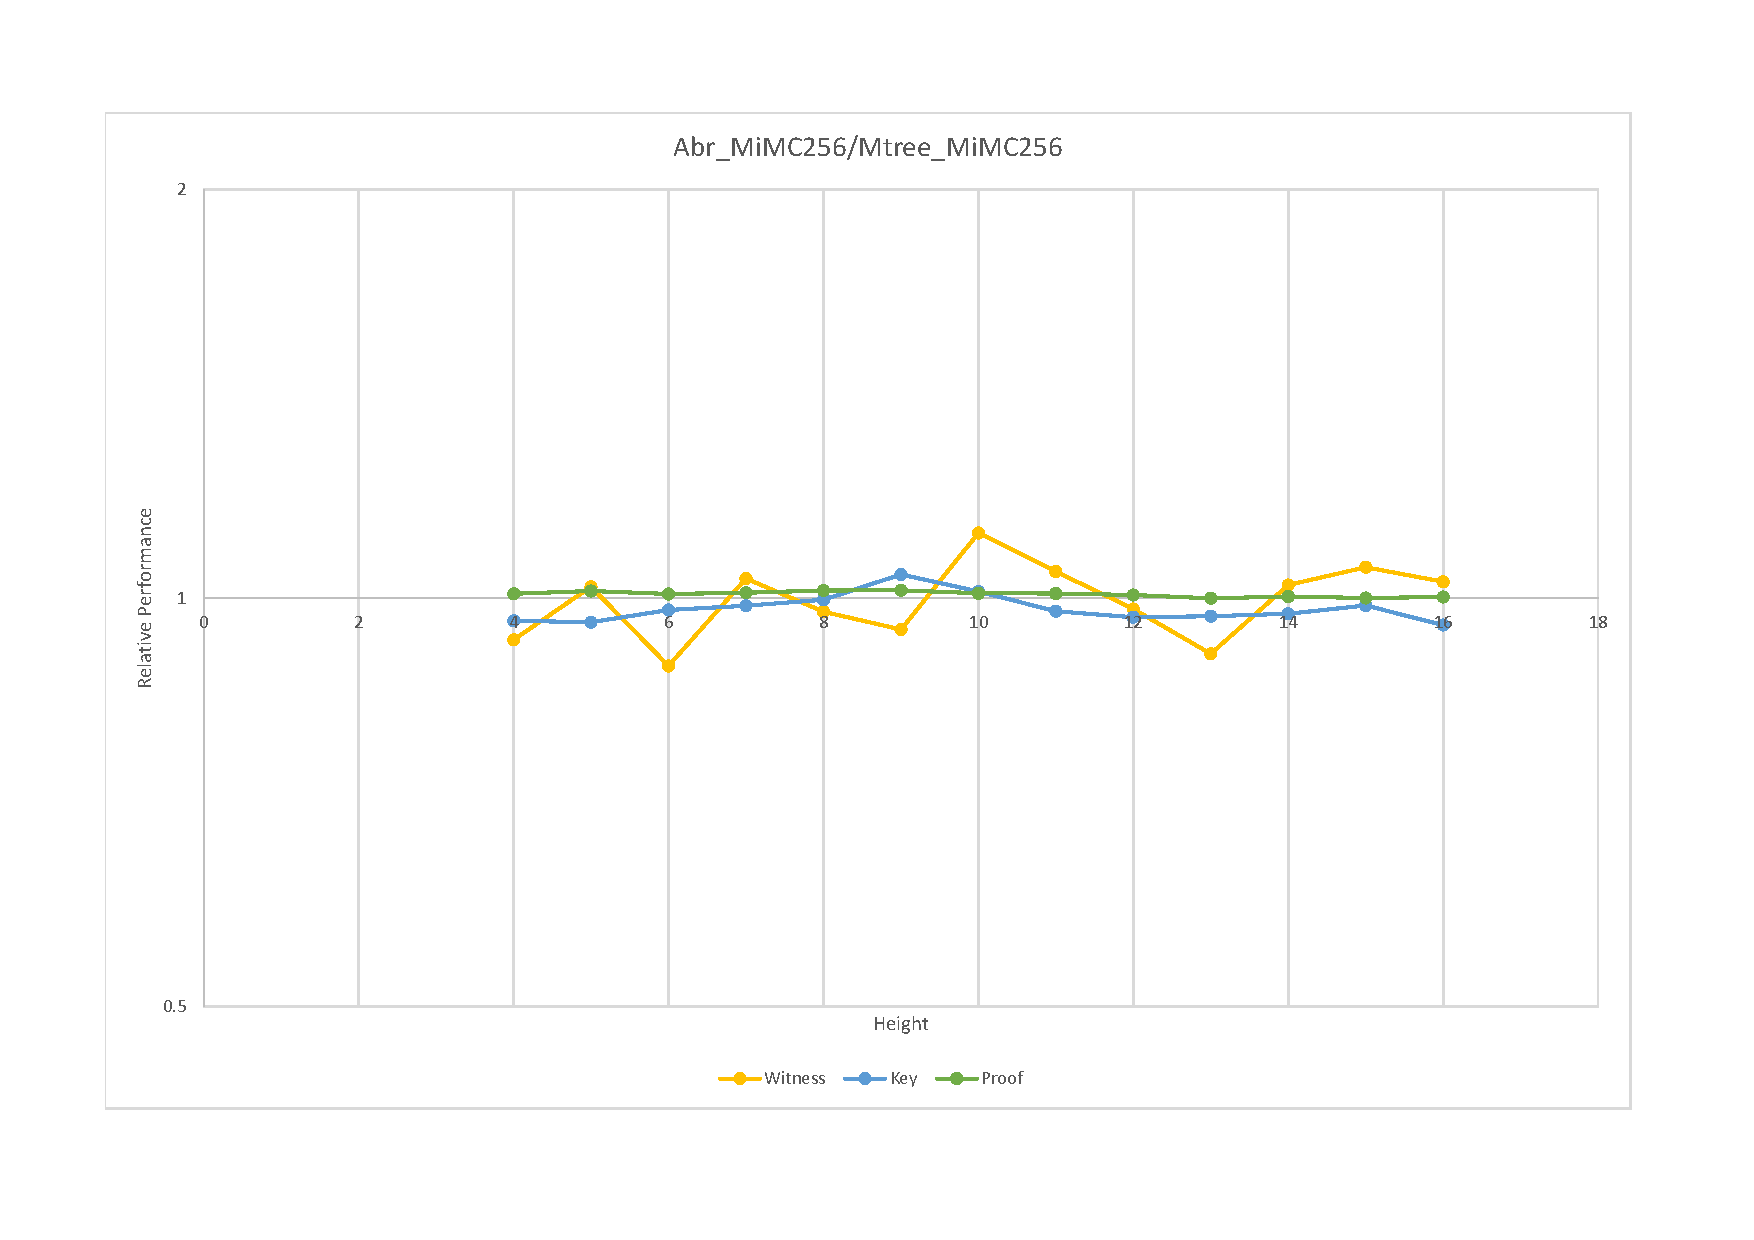
\includegraphics[scale=0.33]{res/mtree_vs_abr.pdf}
	\caption{Relative performance of path verification over ABRs compared to Merkle Trees using
		MiMC-256; we can see that the difference is negligible.}\label{fig:mtree_vs_abr}
\end{figure}

Finally, in Figure~\ref{fig:mtree_vs_abr} we compared the performance of path verification over
ABRs compared to Merkle Trees when using a field-native CHF like MiMC-256.
The difference, as expected, is negligible, and even for non-native functions like SHA-256, the
Merkle Tree is about 10--20\% faster than the ABR\@.
